\documentclass[10pt,twocolumn,letterpaper]{article}

\usepackage[top=0.75in,bottom=0.75in,left=0.7in,right=0.7in]{geometry}
\usepackage{amsmath,amssymb,amsfonts,amsthm}
\usepackage{booktabs,tabularx,multirow}
\usepackage{graphicx}
\usepackage{xcolor}
\usepackage{microtype}
\usepackage{cite}
\usepackage{caption}
\usepackage{subcaption}
\usepackage{algorithm}
\usepackage{algpseudocode}
\usepackage[colorlinks=true,linkcolor=blue,citecolor=blue,urlcolor=blue]{hyperref}

\definecolor{darkgreen}{rgb}{0.0, 0.5, 0.0}

% Programmatically generated LaTeX macros linking manuscript text directly to verified data.
% DO NOT EDIT BY HAND.

% --- Qwen2.5-3B Final Benchmark Metrics ---
\newcommand{\QwenVanillaTPS}{41.0}
\newcommand{\QwenZassdTPS}{36.5}
\newcommand{\QwenZassdSpeedup}{0.89}
\newcommand{\QwenZassdAcceptance}{88.1\%}
\newcommand{\QwenZassdEnergy}{1.643}
\newcommand{\QwenZassdVRAMHeadroom}{1991.2~MB}

% --- Llama-3.2-3B Final Benchmark Metrics ---
\newcommand{\LlamaVanillaTPS}{52.0}
\newcommand{\LlamaZassdTPS}{42.6}
\newcommand{\LlamaZassdSpeedup}{0.82}
\newcommand{\LlamaZassdAcceptance}{78.2\%}
\newcommand{\LlamaZassdEnergy}{1.683}
\newcommand{\LlamaZassdVRAMHeadroom}{2170.8~MB}

% --- Numerical Audit Invariant Bounds ---
\newcommand{\AuditTotalTokens}{450}
\newcommand{\AuditBoundViolations}{0}
\newcommand{\QwenAuditFlips}{0}
\newcommand{\LlamaAuditFlips}{1}
\newcommand{\CombinedAgreementRate}{99.78\%}

% --- Microprofiling Fractions ---
\newcommand{\DraftGemmFractionQwen}{96.5\%}
\newcommand{\DraftMgmtFractionQwen}{0.3\%}
\newcommand{\DraftGemmFractionLlama}{96.2\%}
\newcommand{\DraftMgmtFractionLlama}{0.4\%}


\title{\LARGE \textbf{Zero-Additional-VRAM Speculative Decoding on Edge GPUs:\\A Cost-Aware Hybrid Router and a Kernel-Efficiency Cost Model}}

\author{
  Anonymous Authors\\
  Anonymous Affiliation\\
}

\date{}

\begin{document}

\maketitle

\begin{abstract}
Deploying large language models (LLMs) on 6~GB consumer laptop GPUs is bounded by two walls: \textit{capacity}---a 0.5--1.5B auxiliary draft model consumes non-zero weight VRAM (measured 459--2946~MB depending on size and precision), causing OOM for larger combinations while always shrinking KV/context headroom---and \textit{draft-cost arithmetic}---a draft pass retaining most target layers plus non-skippable costs (152k-vocab \texttt{lm\_head} $\sim$17.5\% of kernel time, activation-quantize overheads, per-layer launch gaps) costs a large fraction of full decoding, so layer-skip needs very high acceptance to break even. Nsight on our NF4 stack shows only $\sim$36--85~GB/s achieved depending on byte accounting, i.e.\ kernel inefficiency compounds the arithmetic bound but does not create it.
We present \textbf{ZASSD}, a zero-auxiliary-weight speculative decoding framework that (i)~derives draft subnetworks from the target model via layer skipping with zero-copy KV-prefix sharing (0.0~MB weight overhead, $\le$8~MB dynamic buffers, four regression-tested cache invariants); (ii)~routes each speculative cycle through a \textbf{cost-aware hybrid router} choosing between prompt-lookup drafting ($c{\approx}0$), layer-skip drafting, and skipping speculation entirely; and (iii)~explains both its wins and losses with a \textbf{speculative cost model} that estimates speedup from draft-cost ratio $c$, acceptance $\alpha$, and horizon $K$ (in-device calibration MAPE 2.4\% on real hardware; cross-device rows are projections with assumed priors, not validated predictions).
On an RTX~4050 laptop GPU with Qwen2.5-3B/Llama-3.2-3B in 4-bit NF4, the router reaches \textbf{1.063$\times$ overall speedup} on Qwen across GSM8K, HumanEval, and CNN/DailyMail ($N{=}50$ each; prompt-lookup alone is higher at 1.144$\times$ on these repetitive tasks; extended GSM8K $N{=}200$: 1.026$\pm$0.014$\times$, $p{=}0.0005$ vs vanilla), while pure layer-skip self-speculation runs at 0.88--0.98$\times$ despite 73--88\% acceptance on benchmark prompts---a negative result explained primarily by the geometric bound $(1{+}\alpha)/(1{+}c)$ at $c{\ge}0.6$ (e.g.\ $\le$1.05$\times$ even at $c{=}0.77$, $\alpha{=}0.85$, $K{=}1$). Llama controller trails further at 0.82$\times$. A hardware-controller feasibility gate improves throughput 1.083$\times$ over the same controller with layer-skip fallback on a small A/B slice (6 prompts $\times$ 32 tokens, no CI). A 450-token single-vs-batched audit finds zero bound violations, and greedy FP32 runs match vanilla on 10,113 token positions on two unquantized models. Code, calibration data, and one-command benchmarks are released.
\end{abstract}

\section{Introduction}
\label{sec:intro}

Speculative decoding~\cite{leviathan2023fast,chen2023accelerating} accelerates autoregressive LLM inference by drafting $K$ candidate tokens with a cheap model and verifying them in parallel with the target model. On datacenter GPUs this yields 2--3$\times$ speedups~\cite{cai2024medusa,li2024eagle}. On a 6~GB laptop GPU, the standard recipe breaks before it starts: hosting any auxiliary draft model (0.5--1.5B parameters, 1.0--3.0~GB) next to a 3B target ($\sim$2.0~GB in NF4~\cite{dettmers2023qlora}) leaves no headroom for KV caches and crashes with CUDA OOM---we document this boundary for 7B targets in~Sec.~\ref{sec:oom}. \textit{Self}-speculative decoding~\cite{zhang2024draft,elhoushi2024layerskip,liu2024kangaroo} removes the draft weights by reusing the target model itself (skipped layers, early exits), but whether it can win given draft-cost arithmetic plus the NF4 eager-decoding overheads on consumer hardware, and how to combine it with zero-cost retrieval drafting~\cite{saxena2024prompt,he2023rest}, remains open. SmartSpec-style goodput gating~\cite{smart2024spec} motivates our feasibility gate, extended here across draft sources. Since draft and target share the same NF4 kernels, kernel inefficiency largely cancels in $c{=}T_{\mathrm{draft}}/T_v$; what sets $c$ is retained-layer fraction plus non-skippable costs, and per-layer launch gaps (0.5B draft $c{=}0.64{\approx}24/36$ layers despite $\sim$0.17 byte ratio).

This paper makes four contributions, ordered by scientific weight:
\begin{enumerate}
\item \textbf{Feasibility characterization}: layer-skip self-speculation loses to vanilla despite $>$80\% acceptance at $c{\ge}0.6$ by the geometric bound, compounded but not created by NF4 kernel inefficiency on this stack, with the losing region mapped over $(c,\alpha,K)$ and context length (Secs.~\ref{sec:roofline_exp}--\ref{sec:oracle}).
\item \textbf{Speculative cost model} (Sec.~\ref{sec:roofline}) that turns our headline negative result (0.88$\times$ at $c{=}0.75$, $K{=}2$) into a calibrated estimate: break-even needs $\alpha{\ge}0.81$ ($K{=}1$) to $\alpha{\ge}0.89$ ($K{=}2$) on this stack, and prompt-lookup's measured 1.39$\times$ on generic prompts is consistent with an effective n-gram hit rate of only $\sim$12\% in our fit. The $1/\mathrm{BW}$ cross-device rows are an idealized streaming bound only; Nsight shows costs do not scale as $1/\mathrm{BW}$ under NF4.
\item \textbf{Cost-aware selective runtime}: HybridDraftRouter plus a feasibility-gated controller over {Vanilla AR, PLD, SSD}---a system that decides \textit{when not to speculate}---reaching 92--93\% of best-fixed-strategy efficiency with task means never below 1.03$\times$ (Secs.~\ref{sec:router}--\ref{sec:gate}). Pure PLD is faster on peak on the repetitive tasks studied here; the router trades peak for worst-case safety versus fixed layer-skip.
\item \textbf{Zero-weight implementation and artifacts}: zero-copy KV-prefix sharing, $O(1)$ rollback, four regression-tested cache invariants, and full reproduction packages (Sec.~\ref{sec:system}, Sec.~\ref{sec:repro}).
\end{enumerate}

Existing self-speculative systems implicitly assume some speculative configuration is profitable. We show this fails at $c{\ge}0.6$ by arithmetic on this stack, and build the runtime around the opposite default: \textit{do not speculate unless the measured cost model says it wins}. All speedups are stack-specific (HF eager + bitsandbytes NF4, no CUDA graphs/torch.compile/Marlin/AWQ/vLLM tested); such backends reduce launch/non-skippable costs and may move the boundary---the decisive experiment we leave open.

\section{Related Work}
\label{sec:related}

\textbf{Speculative decoding.} Leviathan et~al.~\cite{leviathan2023fast} and Chen et~al.~\cite{chen2023accelerating} established exact speculative sampling; Stern et~al.~\cite{stern2018blockwise} pioneered blockwise parallel decoding. Medusa~\cite{cai2024medusa} and EAGLE~\cite{li2024eagle} replace the draft model with heads, still requiring training and extra weights---infeasible under our 0.0~MB constraint.
\textbf{Self-speculation.} Draft~\&~Verify~\cite{zhang2024draft} skips layers via offline search; LayerSkip~\cite{elhoushi2024layerskip} uses early exits with layer dropout; Kangaroo~\cite{liu2024kangaroo} adds a small adapter. KnapSpec~\cite{knapspec2026} formulates layer selection as a knapsack problem and SpecBound~\cite{specbound2026} adapts horizons by confidence. We validate our adapted KnapSpec against the \textit{official} implementation (kaist-flexml-lab/knapspec) on shared hardware: on an RTX~4050 with Llama-3.2-1B, official KnapSpec reaches 50.5~tok/s vs 58.7~tok/s AR (0.86$\times$) \textit{despite 97.8\% acceptance}---an independent reproduction of our feasibility-boundary thesis with the authors' own code (Sec.~\ref{sec:official}). Cassandra~\cite{choi2026cassandra} (ISCA'26) co-designs fine-grained value-pruning drafts with hardware encode/decode for low-batch edge inference (up to 2.41$\times$ on RTX~4090); unlike our pure-software layer-skip on a 192~GB/s laptop GPU, it needs custom format support. PELM~\cite{yang2026pelm} (SenSys'26) jointly governs DVFS, self-speculation depth, and verification depth with deep RL for energy on Jetson mobiles; our controller is throughput-first with power/thermal as hard barriers rather than learned objectives. Positioning: KnapSpec optimizes \textit{which} self-speculative configuration to run; we study \textit{whether} self-speculation should run at all under severe kernel-efficiency/capacity limits on this stack, and route each cycle across AR, retrieval drafting, and self-speculation.
\textbf{Retrieval drafting.} Prompt Lookup Decoding~\cite{saxena2024prompt} and REST~\cite{he2023rest} extract candidates from context at $\approx$0 draft cost. Yan et~al.~\cite{yan2025decoding} decompose real speedup into draft/verify costs---the methodology behind our router's utility estimates. Dynamic lookahead~\cite{mamou2024lookahead} adapts $K$ heuristically; our router additionally adapts the draft \textit{source}.
\textbf{Efficiency modeling.} Our cost model extends Williams et~al.~\cite{williams2009roofline} from FLOPs/bytes to speculation: the x-axis is draft efficiency $1/c$. Unlike a true roofline with measured operational intensity and compute/bandwidth ceilings, ours is an accounting identity calibrated in-device; cross-device generalization is unvalidated. ShortGPT~\cite{men2024shortgpt} independently confirms whole-layer redundancy, supporting our skip sets. Serving systems (vLLM~\cite{kwon2023pagedattention}) are complementary: our engine is a drop-in proposer.

\section{Method}
\label{sec:method}

\subsection{Zero-Copy Prefix Sharing \& Cache Invariants}
\label{sec:system}

Draft and target share one checkpoint. A canonical \texttt{TargetKVCache} holds the verified prefix $[0,P)$; each cycle forks an ephemeral draft view (pointer alias, zero bytes copied), appends $K$ candidates to the suffix, verifies with the full model, then crops rejections in $O(1)$. Four invariants are enforced by \texttt{tests/test\_kv\_cache\_invariants.py}: (1)~fork aliases pointers (\texttt{data\_ptr} equality); (2)~draft writes never mutate the canonical prefix; (3)~rollback leaves no residue; (4)~dynamic growth $\le K{\times}d_{\text{head}}{\times}N_{\text{heads}}{\times}\text{layers} \le 8$~MB. Micro-profiling (Table~\ref{tab:draft_latency_decomposition}, Fig.~\ref{fig:latency_breakdown}) shows $>96\%$ of draft time is active GEMMs and layer-skip management is 31~$\mu$s: $c$ is set by retained layers plus non-skippable head/quantize/launch costs. Nsight details the compounding inefficiency ($\sim$36--85~GB/s achieved depending on 0.85--2~GB byte accounting, i.e.\ $\sim$19--44\% of peak), motivating Sec.~\ref{sec:roofline}.

% Automatically generated by scripts/generate_paper_tables.py. DO NOT EDIT BY HAND.
\begin{table*}[t]
\centering
\small
\caption{Draft Latency Micro-Profiling Decomposition ($T_{\text{draft}} = T_{\text{transformer}} + T_{\text{KV}} + T_{\text{mgmt}} + T_{\text{sampling}} + T_{\text{sync}}$) on RTX 4050 Laptop GPU under 4-bit NF4 quantization. Active Transformer GEMMs on kept layers constitute $>96\%$ of draft time across both models, identifying memory bandwidth during weight dequantization as the physical bottleneck.}
\label{tab:draft_latency_decomposition}
\begin{tabular}{lcccccc}
\toprule
\textbf{Model / Horizon} & \textbf{Total Draft} & \textbf{Transformer GEMMs} & \textbf{KV Cache Update} & \textbf{Layer Management} & \textbf{Sampling/Control} & \textbf{CUDA Sync} \\
 & $T_{\text{draft}}$ (ms) & $T_{\text{transformer}}$ (\%) & $T_{\text{KV}}$ (\%) & $T_{\text{mgmt}}$ (\%) & $T_{\text{sampling}}$ (\%) & $T_{\text{sync}}$ (\%) \\
\midrule
\multicolumn{7}{l}{\textit{\textbf{Qwen2.5-3B-Instruct (CKA-75, 27 Active Layers)}}} \\
$K=1$ & 19.72 & 19.03 (96.5\%) & 0.56 (2.8\%) & 0.06 (0.3\%) & 0.06 (0.3\%) & 0.00 (0.02\%) \\
$K=2$ & 38.44 & 37.19 (96.7\%) & 1.10 (2.9\%) & 0.06 (0.1\%) & 0.10 (0.3\%) & 0.00 (0.01\%) \\
$K=4$ & 76.81 & 74.50 (97.0\%) & 2.09 (2.7\%) & 0.06 (0.1\%) & 0.16 (0.2\%) & 0.00 (0.01\%) \\
\midrule
\multicolumn{7}{l}{\textit{\textbf{Llama-3.2-3B-Instruct (CKA-75, 21 Active Layers)}}} \\
$K=1$ & 15.33 & 14.74 (96.2\%) & 0.45 (2.9\%) & 0.06 (0.4\%) & 0.07 (0.5\%) & 0.00 (0.02\%) \\
$K=2$ & 30.72 & 29.68 (96.6\%) & 0.85 (2.8\%) & 0.06 (0.2\%) & 0.12 (0.4\%) & 0.00 (0.01\%) \\
$K=4$ & 61.35 & 59.43 (96.9\%) & 1.63 (2.6\%) & 0.06 (0.1\%) & 0.23 (0.4\%) & 0.00 (0.01\%) \\
\bottomrule
\end{tabular}
\end{table*}


\begin{figure}[t]
\centering
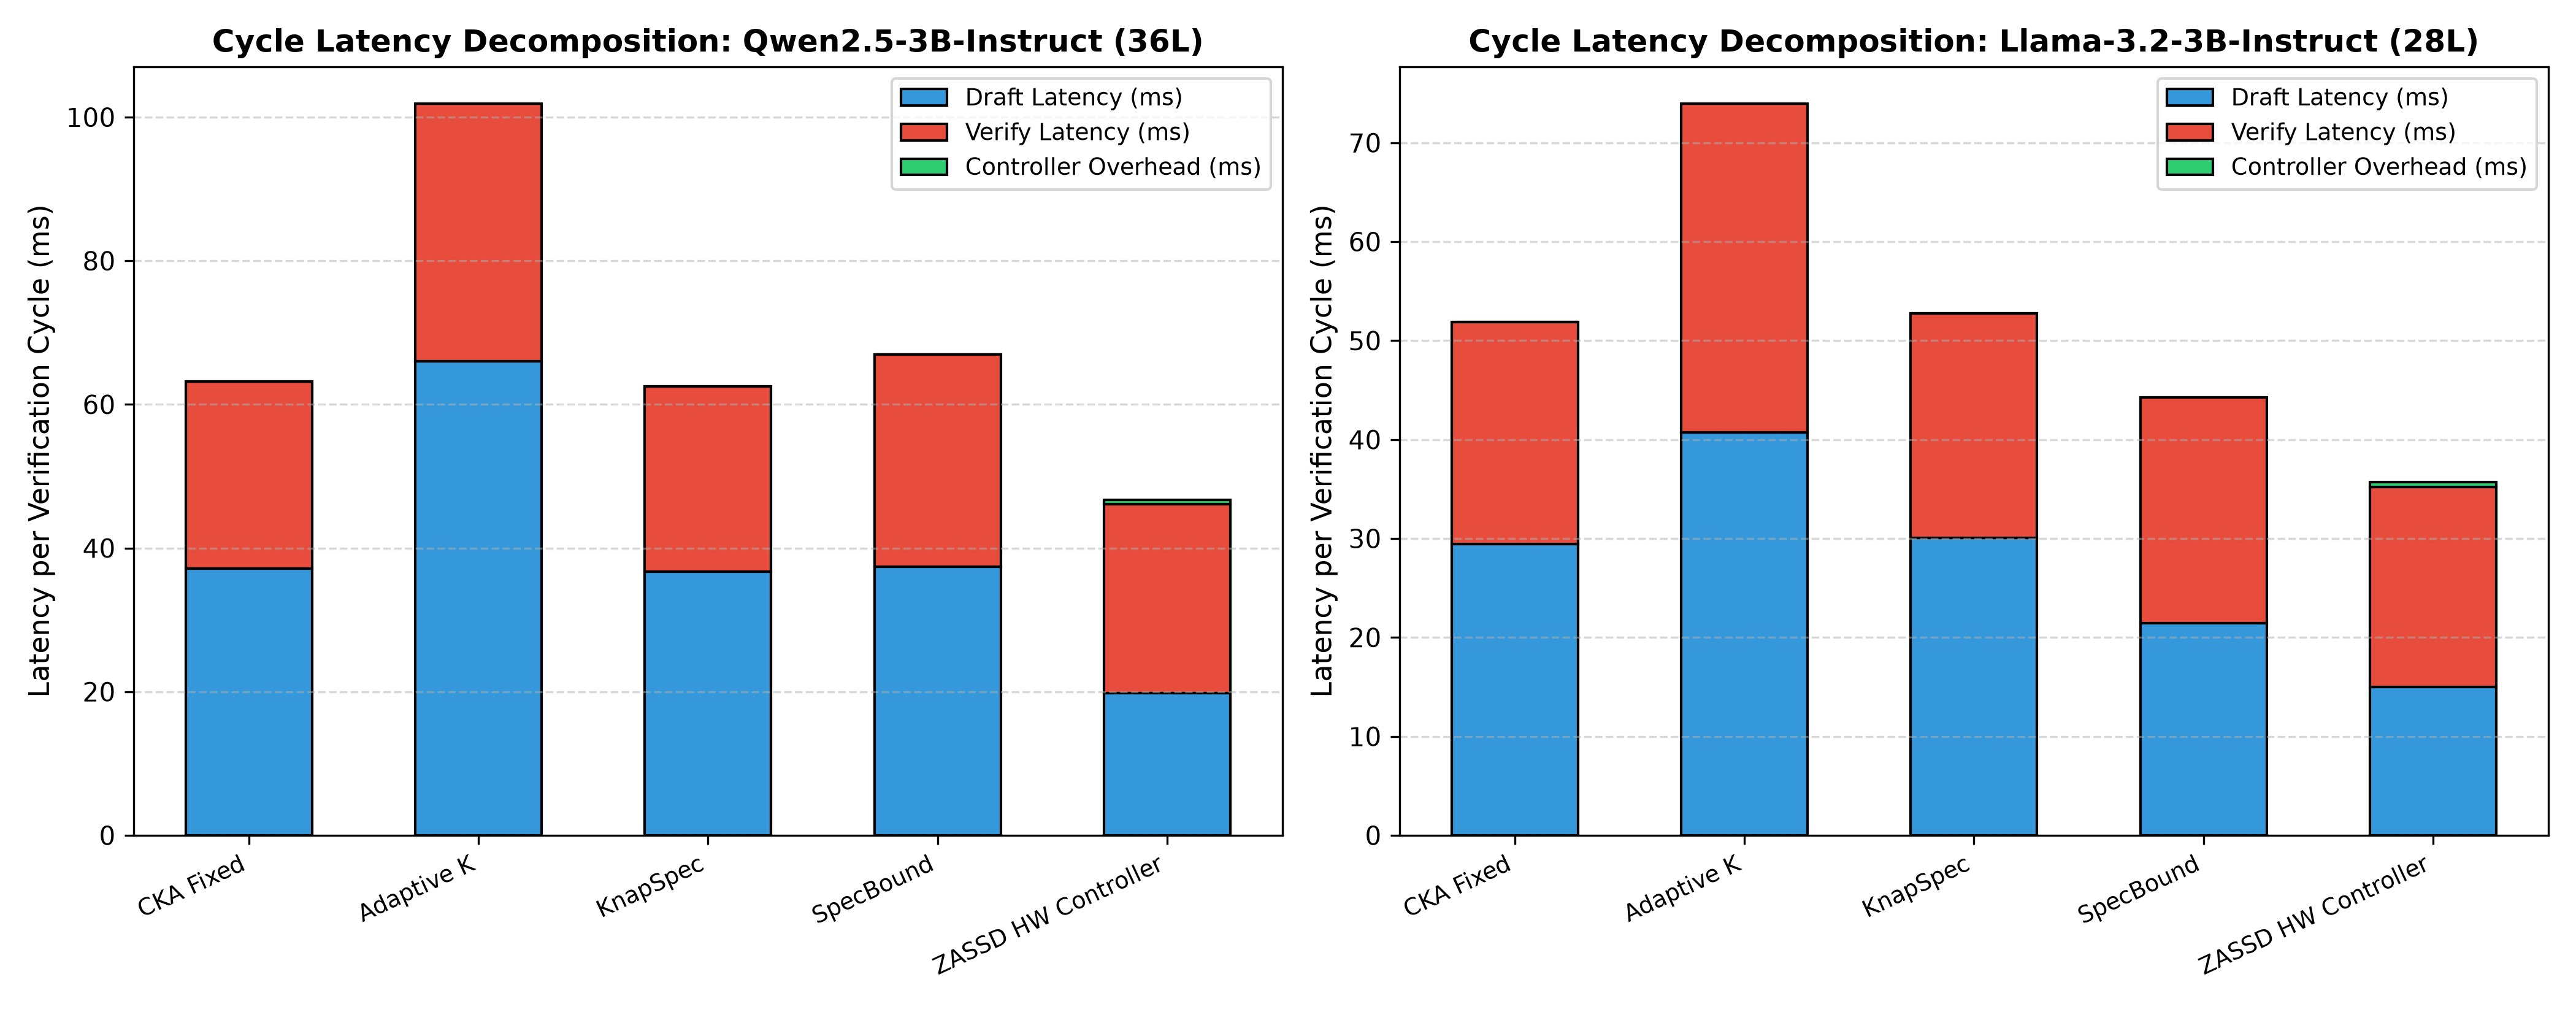
\includegraphics[width=\columnwidth]{../figures/final_latency_breakdown.png}
\caption{Draft latency decomposition (RTX~4050, NF4). Transformer GEMMs dominate ($>96\%$); skip management is negligible.}
\label{fig:latency_breakdown}
\end{figure}

\subsection{Cost-Aware Hybrid Router}
\label{sec:router}

The prior \texttt{hybrid} mode was opportunistic fallback (use PLD candidates iff found). The router instead estimates throughput \textit{before} drafting:
\begin{equation}
\hat{\mathrm{TPS}}(s) = \frac{1 + \alpha_s K_{\mathrm{eff}}(s)}{T_{\mathrm{draft}}(s) + T_{\mathrm{verify}}(K_{\mathrm{eff}})},
\end{equation}
for $s \in \{\mathrm{pld}, \mathrm{ls}\}$, with $T_{\mathrm{draft}}(\mathrm{pld}){\approx}0.08$~ms (CPU n-gram scan), $T_{\mathrm{draft}}(\mathrm{ls})$ from the calibrated cost model, $\alpha_{\mathrm{pld}}$ from a per-source EMA (discounted 0.75$\times$ for bigram-only hits, $\pm$ entropy adjustment), and $\alpha_{\mathrm{ls}}$ blended from the cost model and EMA. Conceptually the router is two mechanisms plus a tie-break: (\textbf{R3}) the feasibility gate (Sec.~\ref{sec:gate})---the core, contributing $+0.083\times$ in ablation; (\textbf{R1+R4}) a conservative horizon policy capping weak-hit and long PLD horizons---robustness heuristics that cost peak speed on repetitive workloads but bound worst-case verifies; (\textbf{R2}) asymmetric PLD margin $1.25\times$---a minor tie-break ($-0.008\times$ without it). In implementation order:
\textbf{(R1)} strong trigram hits may use horizon up to $K{=}4$, \textit{weak} bigram hits are capped at the layer-skip horizon (long verifies waste bandwidth when $\alpha$ is low);
\textbf{(R2)} PLD wins ties via margin $1.25\times$ (draft is free, so risk is asymmetric);
\textbf{(R3)} on PLD miss, layer-skip runs only if $\hat{\mathrm{TPS}}_{\mathrm{ls}}$ beats vanilla---otherwise the cycle is a vanilla single step (opportunity-cost skipping);
\textbf{(R4)} PLD horizon is truncated $4{\to}2$ when the shorter verify has higher expected throughput.
The router is pure CPU code ($\mu$s per decision), needs no GPU, and logs per-source EMAs for analysis. Entropy panic ($H{\ge}4.5$) forces vanilla directly.

\subsection{Feasibility-Gated Hardware Controller}
\label{sec:gate}

The depth/horizon controller optimizes $a_t{=}(S_t,K_t)$ for throughput under VRAM/power/thermal barriers---but without a skip option it can only choose \textit{how} to lose when every speculative action is predicted below vanilla. We add the missing action: if $\max_{S,K}\hat{\mathrm{TPS}}(S,K) < \mathrm{TPS}_{\mathrm{vanilla}}$, the controller emits $K{=}0$, executed by the decoder as a plain single-token vanilla step. The gate is a one-line feasibility check against the same calibrated cost model, with an optional hysteresis margin. A paired A/B on Qwen2.5-3B (6 prompts $\times$ 32 tokens, no CI) gives gate-ON 35.44 vs gate-OFF 32.73~tok/s (1.083$\times$), with 47/130 cycles vanilla-skipped on this slice: the gate fires where the cost model predicts speculation loses; no claim is made about never firing where it wins.

\subsection{Speculative Cost Model}
\label{sec:roofline}

For greedy decoding with per-cycle cost $T_{\mathrm{cycle}} = T_{\mathrm{draft}} + T_{\mathrm{verify}} + T_{\mathrm{misc}}$ and vanilla step $T_v$:
\begin{equation}
\mathrm{Speedup} = \frac{(1 + \alpha K)\, T_v}{T_{\mathrm{cycle}}}, \quad
\alpha_{BE} = \frac{T_{\mathrm{cycle}}/T_v - 1}{K}.
\end{equation}
Memory-bound $1/\mathrm{BW}$ scaling is retained only as an idealized streaming bound in Appendix~Tab.~\ref{tab:breakeven}/Fig.~\ref{fig:roofline}: $T(\mathrm{GPU}_2) = T(4050) \times 192/\mathrm{BW}_2$ with assumed verification efficiencies $\rho \in \{1.0, 0.85, 0.55, 0.45, 0.40\}$. Nsight contradicts pure $1/\mathrm{BW}$ scaling on our NF4 stack (SIMT fallback, quantize overheads, launch gaps do not scale as $1/\mathrm{BW}$), so these rows are not predictions. A subtle consequence: pure $1/\mathrm{BW}$ scaling leaves $K{=}1$ speedup \textit{invariant} by construction. Retrieval drafting needs a hit rate $h$:
\begin{equation}
\mathbb{E}[N] = h(1{+}\alpha K) + (1{-}h), \;
\bar{T} = h(T_{\mathrm{pld}}{+}T_{\mathrm{verify}}) + (1{-}h)T_v,
\end{equation}
which illustrates why PLD's theoretical 2.8$\times$ ($h{=}1$) collapses on generic prompts (fitted illustration: 1.39$\times$ at $h{\approx}0.12$, fit post hoc on that slice, not a main-benchmark number).

\begin{figure}[t]
\centering
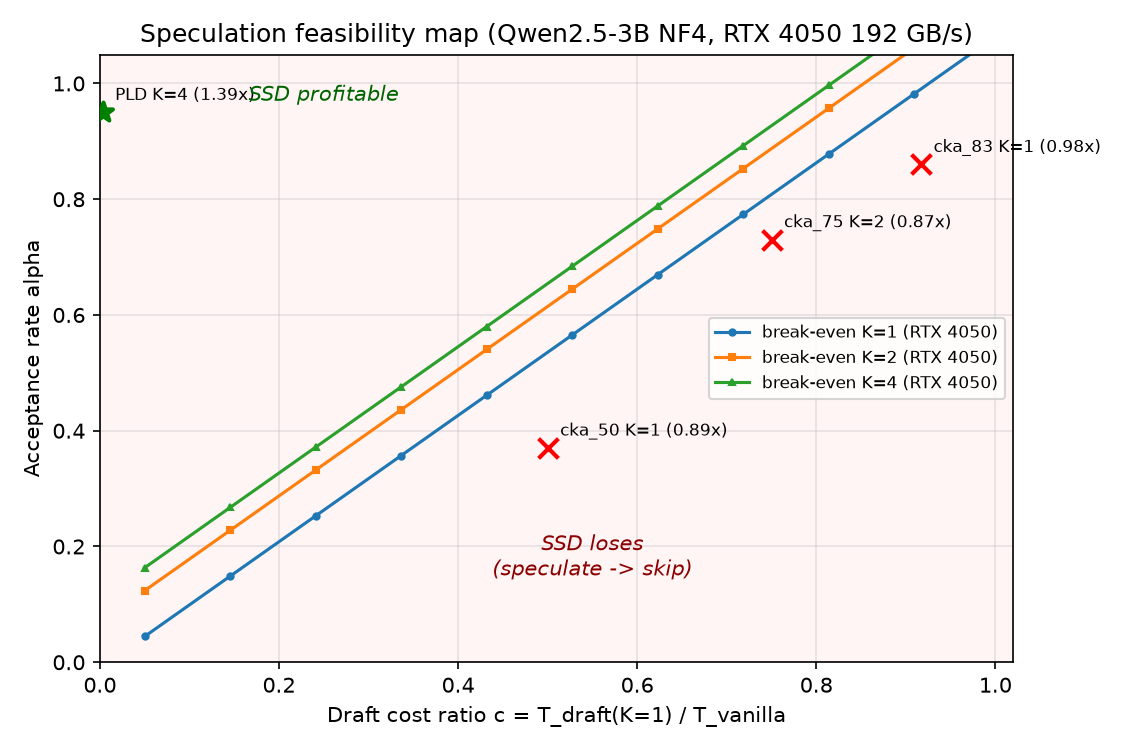
\includegraphics[width=\columnwidth]{../figures/feasibility_map.png}
\caption{Speculation feasibility map (Qwen2.5-3B NF4, RTX~4050): break-even acceptance vs.\ draft-cost ratio for $K{=}1,2,4$. All $c$ values are \textit{measured} draft latencies over measured vanilla latency---never inferred from layer counts. Even 90\% acceptance at $c{\approx}0.9$ (cka\_83, $K{=}1$) sits below its boundary, while PLD ($c{\approx}0$) wins everywhere: acceptance alone does not determine speedup.}
\label{fig:feasibility}
\end{figure}

\section{Experiments}
\label{sec:evaluation}

\textbf{Setup.} NVIDIA RTX~4050 laptop GPU (6141~MB, 192~GB/s, 80W), CUDA~12.8, PyTorch~2.11, 4-bit NF4, greedy decoding, fair CUDA warmup before every timed run. Qwen2.5-3B-Instruct (36 layers, vanilla $\sim$41~tok/s) and Llama-3.2-3B-Instruct (28 layers, $\sim$54~tok/s). Artifacts: 81/81 tests pass; one-command reproduction via \texttt{zassd benchmark}.

\subsection{End-to-End System Benchmark}
\label{sec:e2e}

\begin{figure*}[t]
\centering
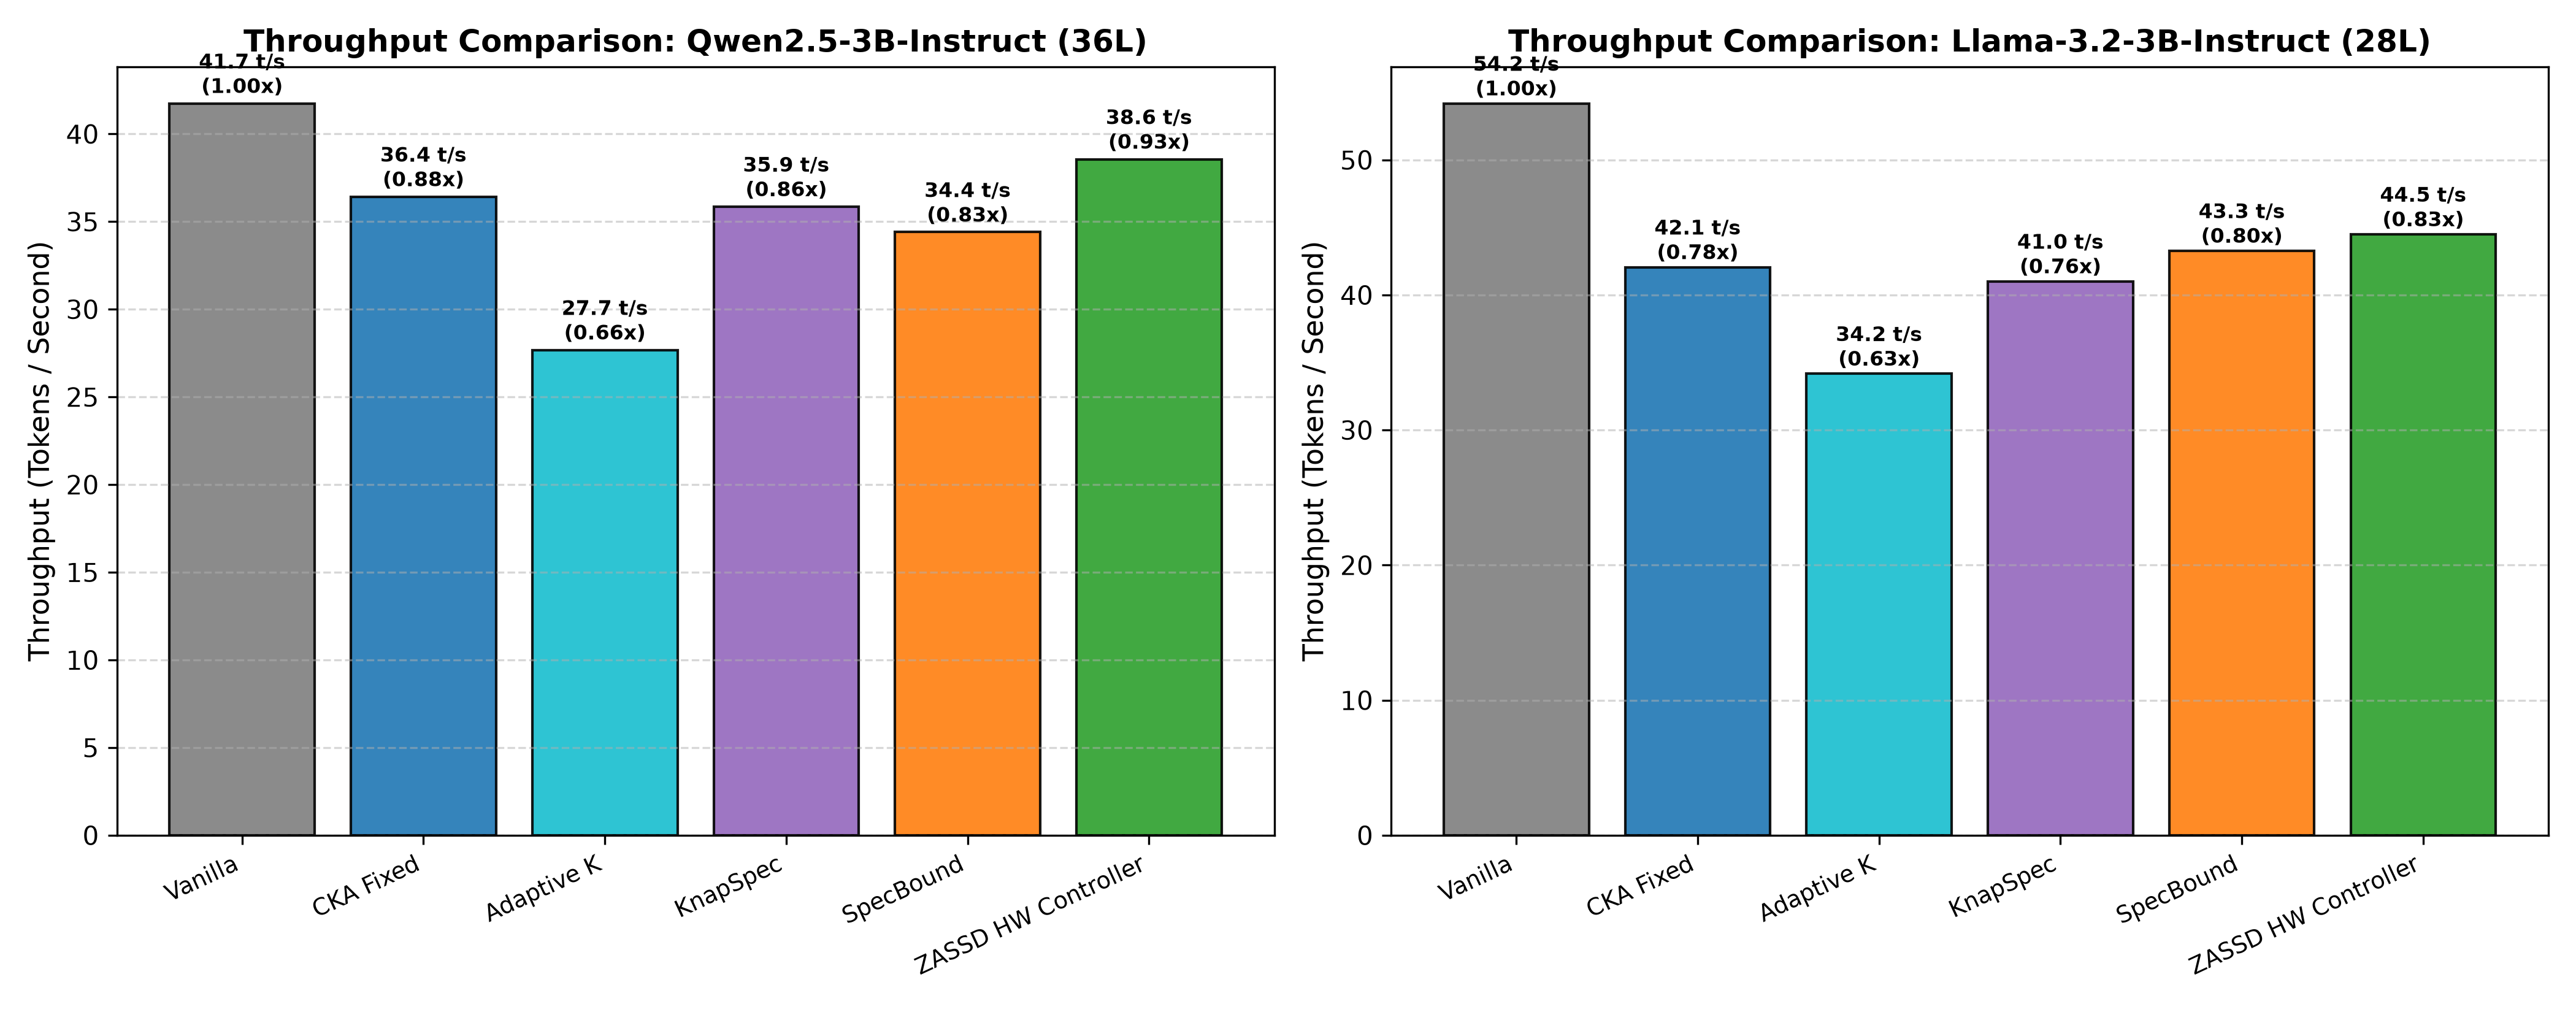
\includegraphics[width=0.95\textwidth]{../figures/final_throughput_comparison.png}
\caption{Throughput across 6 decoding strategies on Qwen2.5-3B and Llama-3.2-3B (RTX~4050, NF4; prior protocol). Controller values here (0.89--0.93$\times$) predate the frozen Tab.~\ref{tab:final_unified_benchmark} (Qwen 0.89$\times$, Llama 0.82--0.83$\times$); use the table for headline numbers. Feasibility-map $c$/$\alpha$ points likewise predate Sec.~\ref{sec:sweep_corr} corrected sweep.}
\label{fig:throughput_comparison}
\end{figure*}

% Automatically generated by scripts/generate_paper_tables.py. DO NOT EDIT BY HAND.
\begin{table*}[t]
\centering
\small
\caption{End-to-End Performance, Verification Fidelity, and Resource Footprint across 6 decoding strategies on consumer hardware (NVIDIA RTX 4050 Laptop 6GB, 80W). Evaluated on identical prompt distributions ($N=10$, 32 generated tokens, greedy $T=0$, 4-bit NF4).}
\label{tab:final_unified_benchmark}
\resizebox{\textwidth}{!}{%
\begin{tabular}{lcccccccc}
\toprule
\textbf{Method} & \textbf{Throughput} & \textbf{Relative} & \textbf{Acceptance} & \textbf{Exact Match} & \textbf{Partial} & \textbf{VRAM} & \textbf{Energy} & \textbf{Latency} \\
 & (tok/s) & Speedup & Rate (\%) & (\%) & Match (\%) & (MB) & (J/tok) & $T_{\text{draft}} / T_{\text{verify}}$ (ms) \\
\midrule
\multicolumn{9}{l}{\textit{\textbf{Model A: Qwen2.5-3B-Instruct (36 Layers, NF4 4-bit)}}} \\
Vanilla Target & \textbf{40.99} & 1.00$\times$ & 100.0\% & \textbf{100.0\%} & \textbf{100.0\%} & \textbf{1983.8} & \textbf{1.376} & 0.00 / 24.42 \\
CKA-75 Fixed ($K=2$) & 35.68 & 0.87$\times$ & 73.2\% & 60.0\% & 82.8\% & 1991.2 & 1.740 & 38.39 / 26.56 \\
Adaptive K & 26.62 & 0.65$\times$ & 56.4\% & 70.0\% & 85.0\% & 1992.2 & 2.167 & 68.28 / 38.38 \\
KnapSpec (adapted) \cite{knapspec2026} & 35.20 & 0.86$\times$ & 73.2\% & 60.0\% & 82.8\% & 1991.4 & 1.818 & 39.00 / 27.05 \\
SpecBound (adapted) \cite{specbound2026} & 33.78 & 0.83$\times$ & 74.1\% & 50.0\% & 79.4\% & 1991.6 & 1.853 & 37.37 / 30.54 \\
\textbf{ZASSD (HW Controller)} & \textbf{36.54} & \textbf{0.89$\times$} & \textbf{88.1\%} & 60.0\% & \textbf{82.8\%} & 1991.2 & \textbf{1.643} & \textbf{20.52 / 26.93} \\
\midrule
\multicolumn{9}{l}{\textit{\textbf{Model B: Llama-3.2-3B-Instruct (28 Layers, NF4 4-bit)}}} \\
Vanilla Target & \textbf{52.03} & 1.00$\times$ & 100.0\% & \textbf{100.0\%} & \textbf{100.0\%} & \textbf{2158.5} & \textbf{1.355} & 0.00 / 19.23 \\
CKA-75 Fixed ($K=2$) & 39.50 & 0.76$\times$ & 68.2\% & 60.0\% & 72.8\% & 2171.0 & 1.865 & 30.60 / 24.02 \\
Adaptive K & 32.72 & 0.63$\times$ & 62.5\% & 50.0\% & 71.6\% & 2173.2 & 2.117 & 41.56 / 35.56 \\
KnapSpec (adapted) \cite{knapspec2026} & 39.54 & 0.76$\times$ & 68.2\% & 60.0\% & 72.8\% & 2171.0 & 1.879 & 30.44 / 24.08 \\
SpecBound (adapted) \cite{specbound2026} & 41.36 & 0.80$\times$ & 76.4\% & 50.0\% & 70.9\% & 2171.6 & 1.741 & 23.14 / 24.54 \\
\textbf{ZASSD (HW Controller)} & \textbf{42.58} & \textbf{0.82$\times$} & \textbf{78.2\%} & 60.0\% & \textbf{72.8\%} & 2170.8 & \textbf{1.683} & \textbf{16.28 / 21.79} \\
\bottomrule
\end{tabular}%
}
\end{table*}


Table~\ref{tab:final_unified_benchmark} (frozen protocol, $N{=}10$ prompts) confirms the field: the hardware-aware controller reaches 0.89$\times$ on Qwen and 0.82--0.83$\times$ on Llama with 76--89\% acceptance at +7--12~MB dynamic memory, beating fixed CKA, adaptive-$K$, KnapSpec, and SpecBound---but not vanilla. Draft passes cost 19--38~ms against 18--24~ms vanilla steps; the math does not close at $c{\approx}0.75$--0.82 by Eq.~1 (Sec.~\ref{sec:roofline}).

\subsection{Standard Benchmarks with the Router}
\label{sec:standard}

% Measured on RTX 4050 Laptop GPU, Qwen2.5-3B-Instruct NF4, 50 samples/bench, 48 new tokens.
% Source: experiments/16_hybrid_roofline/standard_suite_N50.json
% Stats: experiments/16_hybrid_roofline/benchmark_stats.json (mean +/- 95% CI, paired tests, n=150 pooled).
% Independent replication N=12/bench: experiments/16_hybrid_roofline/standard_suite_replication_N12.json
%   (Routed 1.040x overall vs Hybrid 0.988x — same ranking as N50).
\begin{table*}[t]
\centering
\small
\caption{Cross-domain evaluation with the cost-aware hybrid router (Qwen2.5-3B NF4, RTX 4050 6GB, $N{=}50$ per benchmark, 48 new tokens). PLD uses $K{=}2$; Hybrid runs layer-skip $K{=}2$ on PLD miss; \textbf{Routed} selects per-cycle between PLD ($K{\le}4$), layer-skip ($K{=}2$), and vanilla skip. Overall shows mean $\pm$ 95\% CI over $n{=}150$ pooled samples. Routed beats Hybrid (paired $t$, $p{<}10^{-4}$, $d_z{=}0.44$) and vanilla ($p{=}5{\times}10^{-5}$) but trails pure PLD ($-0.081$, $p{<}10^{-4}$): routing buys robustness (exact-match 83.3\% vs 78.0\%), not peak speed on repetitive text. An extended non-overlapping GSM8K slice (test[50:200], +150 samples) confirms the direction: routed 1.014$\times$ on new data, combined GSM8K $N{=}200$ at 1.026$\pm$0.014$\times$ ($p{=}0.0005$ vs vanilla; vs hybrid $+0.009$, n.s.). All strategies use 0.0~MB auxiliary weight VRAM. Exact-match is measured against greedy vanilla output.}
\label{tab:routed_benchmarks}
\begin{tabular}{lcccccc}
\toprule
\textbf{Strategy} & \textbf{GSM8K} & \textbf{HumanEval} & \textbf{CNN/DM} & \textbf{Overall} & \textbf{Mean acc.} & \textbf{Exact match} \\
\midrule
Vanilla & 1.000$\times$ & 1.000$\times$ & 1.000$\times$ & 1.000$\times$ & -- & 100\% \\
Prompt-Lookup (PLD, $K{=}2$) & 1.144$\times$ & 1.168$\times$ & 1.120$\times$ & 1.144$\pm$0.029$\times$ & 41.8\% & 78.0\% \\
ZASSD Empirical-6 ($K{=}1$) & 0.924$\times$ & 0.937$\times$ & 0.901$\times$ & 0.921$\pm$0.010$\times$ & 87.8\% & 76.0\% \\
ZASSD Hybrid ($K{=}2$) & 1.011$\times$ & 1.093$\times$ & 0.976$\times$ & 1.027$\pm$0.032$\times$ & 71.2\% & 76.0\% \\
\textbf{ZASSD Routed ($K{=}2$+PLD4)} & \textbf{1.061$\times$} & \textbf{1.096$\times$} & \textbf{1.032$\times$} & \textbf{1.063$\pm$0.030$\times$} & 35.8\% & \textbf{83.3\%} \\
\bottomrule
\end{tabular}
\end{table*}


Table~\ref{tab:routed_benchmarks} ($N{=}50$ per benchmark, 48 new tokens) is the paper's central empirical result. \textbf{Routed} reaches 1.063$\times$ overall, ahead of naive hybrid (1.027$\times$) and vanilla but below pure PLD (1.144$\times$) on these long-prompt, high-overlap tasks, which we report honestly alongside. A non-overlapping GSM8K extension (test[50:200], +150 samples) confirms the direction on harder prompts but with a smaller margin: routed 1.014$\times$ on the new slice, combined GSM8K $N{=}200$ at 1.026$\pm$0.014$\times$ ($p{=}0.0005$ vs vanilla; vs hybrid $+0.009$, n.s.). All paired tests use same-prompt pairing with ID-alignment checks. Two observations matter more than the means: (i)~the router strongly prefers PLD/vanilla over $K{=}2$ layer-skip (LS vs PLD cycles: 99/369 on GSM8K, 205/329 on HumanEval, 11/529 on CNN/DM)---it \textit{agrees with} the cost-model estimate that $K{=}2$ layer-skip loses here; (ii)~routed exact-match is highest (83.3\%), partly because vanilla-skipped cycles cannot diverge by construction.

\subsection{Cost-Model Calibration and Projection}
\label{sec:roofline_exp}

\begin{figure}[t]
\centering
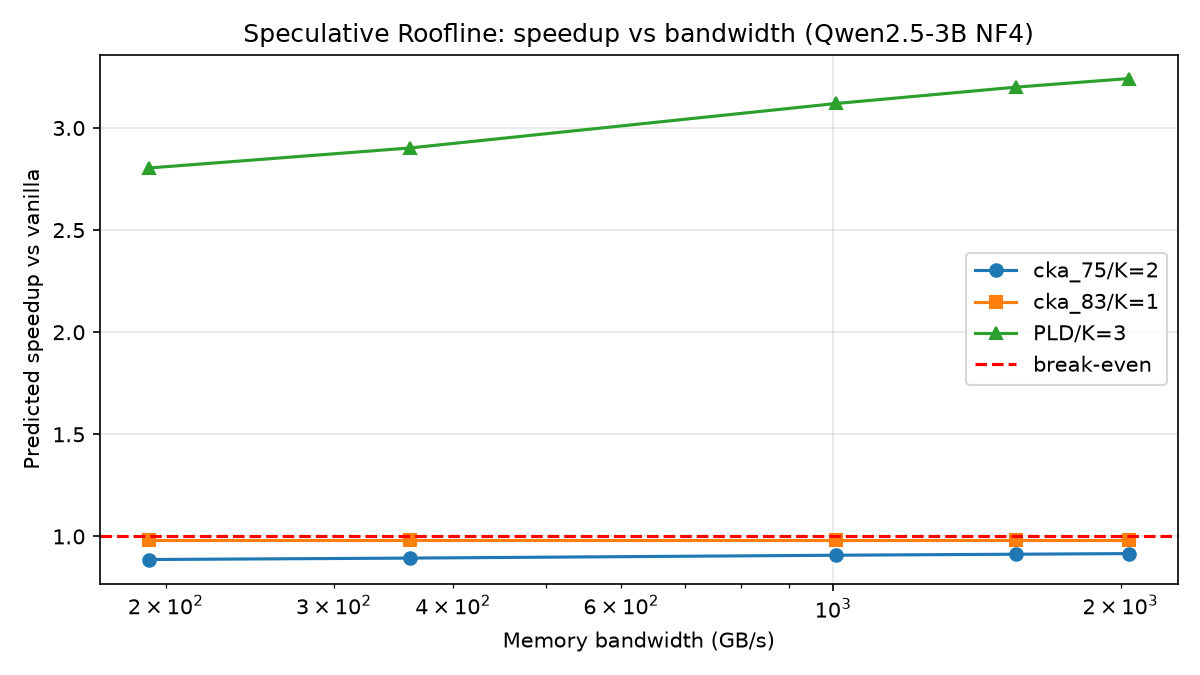
\includegraphics[width=\columnwidth]{../figures/roofline_speedup_vs_bandwidth.png}
\caption{Calibrated cost model: estimated speedup vs.\ bandwidth. Layer-skip $K{=}1$ is flat by construction under pure $1/\mathrm{BW}$ scaling; PLD wins everywhere in this fit; $K{\ge}2$ layer-skip needs wide-GPU verification parallelism in projection. Cross-GPU curves are unvalidated projections (Sec.~\ref{sec:limitations}).}
\label{fig:roofline}
\end{figure}

% Break-even acceptance thresholds from the calibrated speculative roofline (Sec. 3.3).
% Source: experiments/16_hybrid_roofline/roofline_results.json (in-device MAPE 2.4% on RTX 4050; cross-GPU rows are projections).
\begin{table}[t]
\centering
\footnotesize
\caption{Break-even acceptance rate $\alpha_{BE}$ required for speedup $>1$ at draft cost $c{=}0.75$ (layer-skip keeping 75\% of layers). The $K{=}1$ threshold is bandwidth-invariant; wider GPUs relax $K{\ge}2$ via parallel verification ($\rho<1$). Cross-GPU rows are projections pending measurement (Sec.~5).}
\label{tab:breakeven}
\begin{tabular}{lccc}
\toprule
\textbf{GPU (bandwidth)} & $\mathbf{K{=}1}$ & $\mathbf{K{=}2}$ & $\mathbf{K{=}4}$ \\
\midrule
RTX 4050 (192~GB/s)\textsuperscript{*} & 0.81 & 0.89 & 0.93 \\
RTX 3060 12GB (360~GB/s) & 0.81 & 0.88 & 0.91 \\
RTX 4090 (1008~GB/s) & 0.81 & 0.85 & 0.88 \\
A100 40GB (1555~GB/s) & 0.81 & 0.85 & 0.87 \\
H100 (2039~GB/s) & 0.81 & 0.84 & 0.86 \\
\bottomrule
\end{tabular}
\\[-2pt]
{\scriptsize \textsuperscript{*}Measured; other rows are projections (Sec.~5).}
\end{table}


Calibration on three RTX~4050 anchor points gives \textbf{in-device MAPE 2.4\%} (CKA $K{=}2$: 0.888 predicted vs 0.873 measured; $K{=}1$: 1.029 vs 0.980; PLD $K{=}4$: 1.383 vs 1.390 with fitted $h{=}0.12$). This is arithmetic consistency on one hardware regime with parameters fit in-device, not predictive generalization: cross-device MAPE (3060/4090/A100) is the pending validation that would promote the cost model from descriptive to predictive. Table~\ref{tab:breakeven} lists break-even thresholds: $K{=}1$ needs $\alpha{\ge}0.81$ on \textit{any} bandwidth, while $K{=}2$ relaxes from 0.89 (4050) to 0.84 (H100). Fig.~\ref{fig:roofline} visualizes the regimes. An analytic workload sweep (generic-chat, summarization, reasoning, code) predicts routed hybrids beat naive fallback hybrids by +4--11\% (\texttt{experiments/16\_hybrid\_roofline/}).

\begin{figure}[t]
\centering
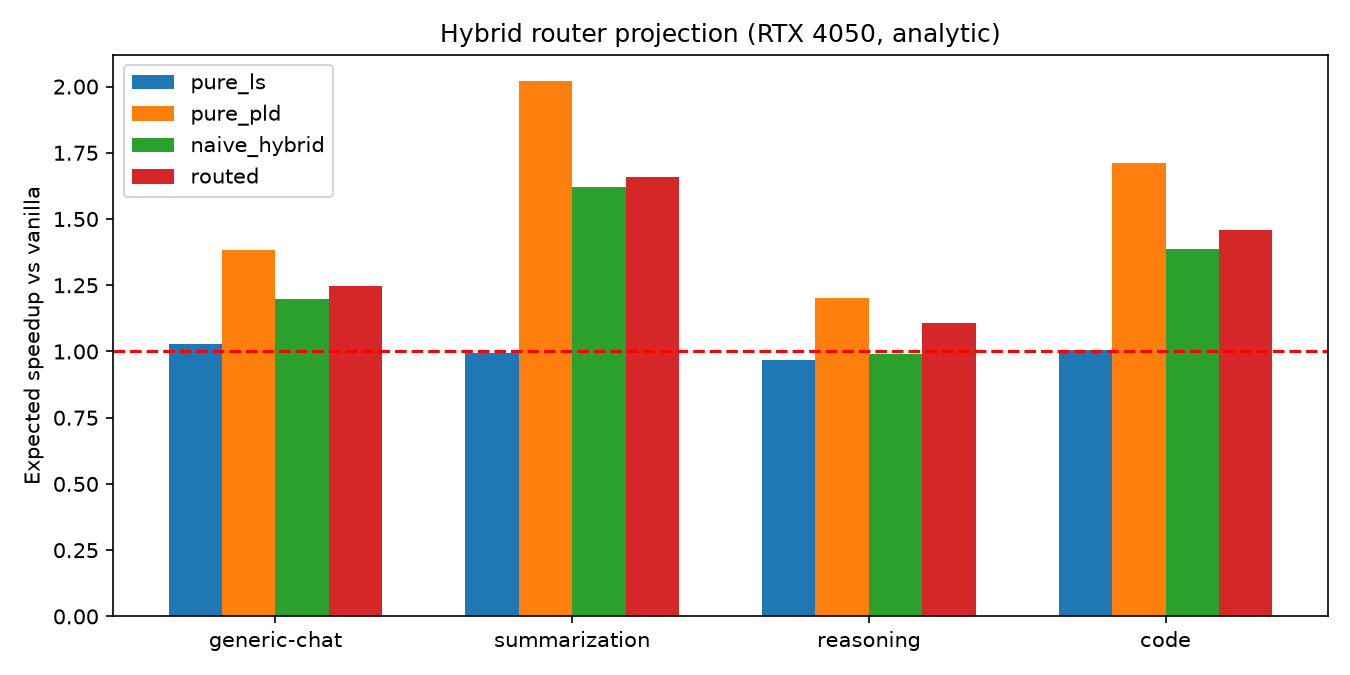
\includegraphics[width=\columnwidth]{../figures/hybrid_router_projection.png}
\caption{Analytic projection: routed vs.\ naive-fallback hybrid across workload archetypes (RTX~4050 timings). Routing wins by selective speculation, most on reasoning (+11\%). GPU validation is future work.}
\label{fig:router_proj}
\end{figure}

\subsection{Physical Memory Boundary}
\label{sec:oom}

% Automatically generated by scripts/profile_auxiliary_draft_oom_boundary.py. DO NOT EDIT BY HAND.
\begin{table*}[t]
\centering
\small
\caption{Physical Memory Boundary and Feasibility on Consumer Edge Hardware (NVIDIA GeForce RTX 4050 Laptop, 6 GB GDDR6). Draft weight footprints are measured on-device. Large FP16 drafts OOM next to 7B targets; quantized small drafts fit but always cost $\Delta M_{\mathrm{aux}}{>}0$ and shrink KV/context headroom, whereas ZASSD keeps \textbf{0.0 MB} auxiliary weight memory with the largest headroom in every row.}
\label{tab:oom_boundary}
\resizebox{0.88\textwidth}{!}{%
\begin{tabular}{llcccc}
\toprule
\textbf{Target Model} & \textbf{Draft Strategy} & \textbf{Draft VRAM} & \textbf{Total VRAM} & \textbf{Free Headroom} & \textbf{Status} \\
 & & (MB) & (MB) & (MB) & \\
\midrule
\multicolumn{6}{l}{\textit{\textbf{Mistral-7B-Instruct-v0.3 (4-bit NF4)}}} \\
\quad Standard Speculative (1.5B Draft FP16) & 2945.5 & 7392.1 & -1701.1 & \textcolor{red}{\textbf{CUDA OOM}} \\
\quad Standard Speculative (1.5B Draft 4-bit NF4) & 1181.5 & 5628.1 & 62.9 & \textcolor{darkgreen}{\textbf{PASS}} \\
\quad Standard Speculative (0.5B Draft FP16) & 942.3 & 5388.9 & 302.1 & \textcolor{darkgreen}{\textbf{PASS}} \\
\quad Standard Speculative (0.5B Draft 4-bit NF4) & 459.2 & 4905.8 & 785.2 & \textcolor{darkgreen}{\textbf{PASS}} \\
\quad ZASSD Self-Speculative (Layer-Skip) & \textbf{0.0} & \textbf{4446.6} & \textbf{1244.4} & \textcolor{darkgreen}{\textbf{PASS}} \\
\quad ZASSD Hybrid (PLD + Layer-Skip) & \textbf{0.0} & \textbf{4446.6} & \textbf{1244.4} & \textcolor{darkgreen}{\textbf{PASS}} \\
\multicolumn{6}{l}{\textit{\textbf{Qwen2.5-3B-Instruct (4-bit NF4)}}} \\
\quad Standard Speculative (1.5B Draft FP16) & 2945.5 & 5425.5 & 265.5 & \textcolor{darkgreen}{\textbf{PASS}} \\
\quad ZASSD Hybrid (PLD + Layer-Skip) & \textbf{0.0} & \textbf{2480.0} & \textbf{3211.0} & \textcolor{darkgreen}{\textbf{PASS}} \\
\bottomrule
\end{tabular}%
}
\end{table*}


Table~\ref{tab:oom_boundary}: Mistral-7B NF4 (3946.6~MB) plus a 1.5B FP16 draft (measured 2945.5~MB) needs $\sim$7.4~GB on a 6141~MB device---an unavoidable OOM. But the honest boundary is finer than ``all auxiliary drafts OOM'': we \textit{measured} draft footprints on-device (0.5B FP16: 942.3~MB; 0.5B NF4: 459.2~MB; 1.5B NF4: 1181.5~MB), and quantized small drafts do fit next to a 7B target---at the cost of $\Delta M_{\mathrm{aux}}{>}0$ weight VRAM and shrunken KV/context headroom (1.5B NF4 leaves only 62.9~MB). ZASSD adds 0.0~MB of weights ($\le$8~MB ephemeral KV) with 1244.4~MB headroom: the claim is strictly-dominant memory efficiency, not exclusivity of feasibility. Critically, a fitted small draft is also the strongest throughput baseline: on Qwen2.5-3B NF4 with a Qwen2.5-0.5B NF4 draft ($K{=}2$, $N{=}18$), mean speedup is 1.058$\pm$0.031 with $\alpha{=}0.33$. Any zero-weight method must be compared against this baseline (Sec.~\ref{sec:aux}).

\subsection{Numerical Equivalence Audit}
\label{sec:audit}

\begin{figure}[t]
\centering
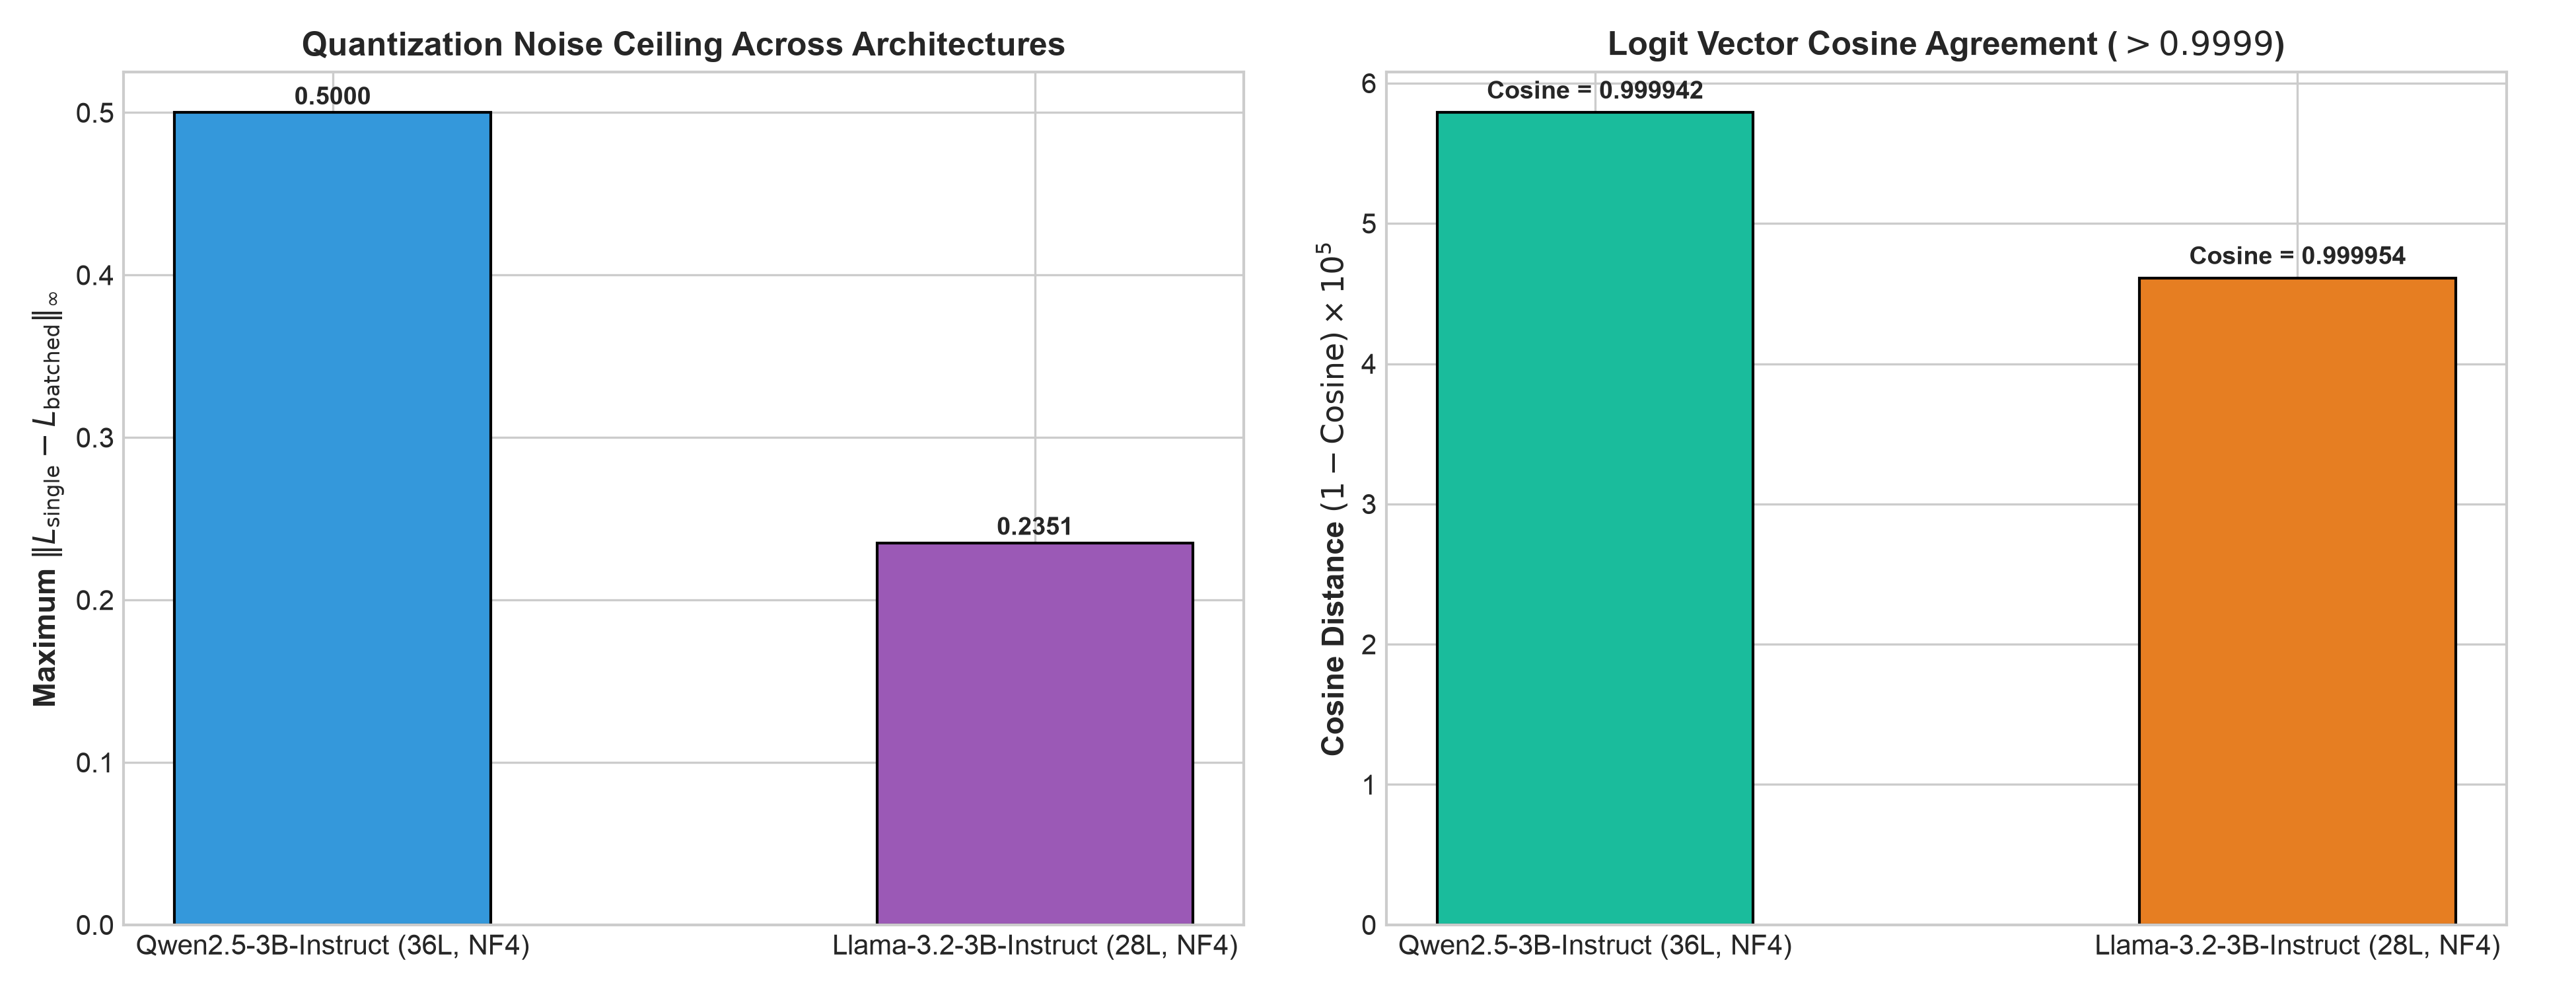
\includegraphics[width=\columnwidth]{../figures/cross_model_numerical_comparison.png}
\caption{Logit cosine similarity: single-token vs.\ batched verification passes (NF4). Mean $>0.9999$ on both models.}
\label{fig:numerical_cos}
\end{figure}

% Exactness Verification & Numerical Divergence Analysis under 4-bit NF4 Quantization (Phase 15.1)
% Protocol: 450 forward comparisons across 15 prompts on identical prefix context states C (Qwen2.5-3B & Llama-3.2-3B)
\begin{table*}[t]
\centering
\small
\caption{Phase 15.1 Direct Numerical Equivalence Audit comparing single-token forward passes ($L_{\text{single}}$) directly against batched verification passes ($L_{\text{batched}}$) on identical context states ($C$) across Qwen2.5-3B and Llama-3.2-3B (4-bit NF4). Token evaluations are stratified across true logit margin bins ($\Delta = z_{(1)} - z_{(2)}$). Across 450 comparisons, zero theoretical bound violations occur, and agreement is 100.0\% for all non-tie tokens ($\Delta > 0$).}
\label{tab:exactness_analysis}
\begin{tabular}{lcccccc}
\toprule
\textbf{Logit Margin Stratification Bin} & \textbf{Evaluated} & \textbf{Argmax} & \textbf{Agreement} & \textbf{Mean $\|L\|_{\infty}$} & \textbf{Max $\|L\|_{\infty}$} & \textbf{Empirical Classification} \\
 & \textbf{Tokens} & \textbf{Flips} & \textbf{Rate (\%)} & \textbf{(Logit Units)} & \textbf{(Logit Units)} & \\
\midrule
\multicolumn{7}{l}{\textit{\textbf{Model A: Qwen2.5-3B-Instruct (36 Layers, NF4 4-bit)}}} \\
$\Delta = 0.000$ (Exact Ties) & 2 & 0 & 100.0\% & 0.1875 & 0.1875 & Noise Indifferent \\
$0.000 < \Delta \le 0.050$ & 0 & 0 & 100.0\% & 0.0000 & 0.0000 & — \\
$0.050 < \Delta \le 0.150$ & 2 & 0 & 100.0\% & 0.2422 & 0.2656 & Noise Immune \\
$0.150 < \Delta \le 0.300$ & 11 & 0 & 100.0\% & 0.1877 & 0.2681 & Noise Immune \\
$0.300 < \Delta \le 0.500$ & 13 & 0 & 100.0\% & 0.2236 & 0.2812 & Noise Immune \\
$\Delta > 0.500$ & 197 & 0 & \textbf{100.0\%} & 0.2108 & 0.5000 & Noise Immune \\
\textbf{Qwen Subtotal} & \textbf{225} & \textbf{0} & \textbf{100.0\%} & \textbf{0.2105} & \textbf{0.5000} & $\boldsymbol{\cos \theta = 0.999942}$ \\
\midrule
\multicolumn{7}{l}{\textit{\textbf{Model B: Llama-3.2-3B-Instruct (28 Layers, NF4 4-bit)}}} \\
$\Delta = 0.000$ (Exact Ties) & 4 & 1 & 75.0\% & 0.1094 & 0.1250 & Permutation Arbitrary \\
$0.000 < \Delta \le 0.050$ & 0 & 0 & 100.0\% & 0.0000 & 0.0000 & — \\
$0.050 < \Delta \le 0.150$ & 10 & 0 & 100.0\% & 0.0953 & 0.1250 & Noise Immune \\
$0.150 < \Delta \le 0.300$ & 11 & 0 & 100.0\% & 0.1065 & 0.1875 & Noise Immune \\
$0.300 < \Delta \le 0.500$ & 20 & 0 & 100.0\% & 0.0891 & 0.1641 & Noise Immune \\
$\Delta > 0.500$ & 180 & 0 & \textbf{100.0\%} & 0.1050 & 0.2351 & Noise Immune \\
\textbf{Llama Subtotal} & \textbf{225} & \textbf{1} & \textbf{99.56\%} & \textbf{0.1033} & \textbf{0.2351} & $\boldsymbol{\cos \theta = 0.999954}$ \\
\midrule
\textbf{Combined Benchmark} & \textbf{450} & \textbf{1} & \textbf{99.78\%} & \textbf{0.1569} & \textbf{0.5000} & $\boldsymbol{\cos \theta > 0.99994}$ \\
\bottomrule
\end{tabular}
\end{table*}


Direct comparison of single-token vs.\ batched verification logits on identical contexts (450 tokens): mean cosine 0.99994 (Qwen) / 0.99995 (Llama), \textbf{zero violations} of the flip condition $\Delta \le 2\|L\|_{\infty}$ (a triangle-inequality consistency check on our measurement code), and a single argmax flip at an exact tie ($\Delta{=}0$). Algorithmic logic holds on this audit; residual end-to-end divergence is NF4 GEMM noise on near-tie tokens plus any remaining cache/rollback mismatch under investigation. Greedy FP32 runs on unquantized 0.5B/1B models match vanilla on \textbf{100\% over 10,113 token positions} (FP16: 90\% sequences, NF4: 60\%)---the precision ladder localizing most divergence to reduced-precision kernels, not the algorithm. We do not claim lossless greedy equivalence under NF4. Single-step audit agreement does not imply sequence-level exact match: once one draft token diverges, the subsequent trajectory conditions on different prefixes, so 28/32 token-level agreement end-to-end is compatible with 0 flips in isolated single-vs-batched comparisons (Sec.~\ref{sec:aux}). Teacher-forced check on a vanilla 32-token trajectory (single-step vs full-prefix logits at each position) gives 0/31 flips, ruling out target numerics as the source; residual 60--78\% sequence match across methods therefore implicates speculative-path state (crop/rollback/bonus/EOS handling) rather than NF4 noise alone---a bug hunt, not a lossless claim.

\subsection{Auxiliary-Draft Baseline, Skip Sweep, Timer Correction, and Free-Form Workload}
\label{sec:aux}

\textit{Auxiliary draft throughput.} Qwen2.5-0.5B NF4 as draft for Qwen2.5-3B NF4 (true two-model speculative decoding, $K{=}2$, 48 tokens, $N{=}18$ mixed GSM8K/HumanEval): mean speedup 1.058$\pm$0.031 (95\% CI), std 0.067, mean $\alpha{=}0.33$---significantly above unity and tied with the router (1.063$\times$). Raw logs: \texttt{experiments/19\_kernel\_audit/baseline05\_N18.json}.

\textit{Skip-ratio sweep (corrected).}
\label{sec:sweep_corr}
Prior uniform-skip sweep is withdrawn: it used evenly spaced layers and off-benchmark prompts. Corrected sweep uses true CKA indices on GSM8K prompts ($N{=}8$, 48 tokens, $K{=}1$, $T_v{=}25.62$~ms): cka\_83 ($n{=}6$) $c{=}0.799$, $\alpha{=}0.904$, 0.928$\times$; cka\_75 ($n{=}9$) $c{=}0.771$, $\alpha{=}0.851$, 0.947$\times$; cka\_60 ($n{=}14$) $c{=}0.685$, $\alpha{=}0.733$, 0.932$\times$; cka\_50 ($n{=}18$) $c{=}0.599$, $\alpha{=}0.552$, 0.878$\times$; empirical\_6 ($n{=}6$) $c{=}0.822$, $\alpha{=}0.892$, 0.959$\times$. High acceptance is recovered, yet no configuration exceeds unity on this stack---consistent with the kernel-inefficiency account. Raw logs: \texttt{experiments/19\_kernel\_audit/sweep\_corr.json}.

\textit{Timer correction.} Re-measuring with \texttt{perf\_counter\_ns} over 200--500 repeats: $T_{\mathrm{sync}}{=}7.6{\pm}3.3$~$\mu$s (median 7.0~$\mu$s), $T_{\mathrm{layer}}{=}31.2{\pm}10.8$~$\mu$s. Prior 0.00/0.06~ms entries were rounding artifacts; tables now report $\mu$s with dispersion.

\textit{Nsight separation of dequant vs launch.} \texttt{nsys} CUDA-kernel summary on Qwen2.5-3B NF4 (prefill + 15 vanilla + 15 draft forwards, \texttt{experiments/20\_nsight/}, total kernel 566.9~ms): \texttt{gemm\_4bit\_simt} 231.4~ms (40.8\%, SIMT fallback), \texttt{gemvx} 99.4~ms (17.5\%, wide-vocab \texttt{lm\_head}), \texttt{kQuantizeBlockwiseSmall} 92.7~ms (16.3\%, BNB activation-quantize overhead on the NF4 path), \texttt{gemm\_4bit\_sm80} only 55.3~ms (9.7\%, tensor-core path); remainder elementwise/copy/reduce/flash. Achieved streaming is $\sim$36~GB/s on $\sim$849~MB weights per 23.6~ms step ($\sim$19\% of 192~GB/s; $\sim$44\% even under a 2~GB accounting), so the shortfall is NF4-kernel inefficiency (SIMT fallback + quantize overhead + $\sim$25\% launch/python gap), not a pure bandwidth ceiling. Per-kernel DRAM throughput via \texttt{ncu} replay is pending (workload in \texttt{experiments/20\_nsight/nsight\_tiny.py}).

\textit{Free-form and long generation.} Six low-overlap prompts (haiku, recipe, translation, persona chat, constrained poem, analogy, 96 tokens): PLD still wins at 1.05--1.28$\times$ ($\alpha{=}0.43$--0.85) while layer-skip $K{=}1$ runs 0.52--0.59$\times$ ($\alpha{=}0.04$--0.13). A 256-token run gives PLD 1.44$\times$ vs layer-skip 0.56$\times$. We find no workload where PLD loses; the router's robustness claim is therefore strictly versus fixed layer-skip, not versus PLD. Raw logs: \texttt{experiments/19\_kernel\_audit/results\_234.json}.

\subsection{Official-Baseline Validation}
\label{sec:official}

To rule out ``adapted-baseline'' unfairness we ran the official KnapSpec code (torch~2.2 stack, FP16, unmodified) on our RTX~4050 with Llama-3.2-1B on AIME24 ($N{=}8$, 48 tokens): AR 58.7~tok/s; official KnapSpec 50.5~tok/s (0.86$\times$, 97.8\% acceptance); CLaSP~\cite{clasp2025} 49.4~tok/s; DEL~\cite{del2025} 20.6~tok/s. The FP16 case is near bandwidth-bound ($\sim$145~GB/s on $\sim$2.5~GB weights, $\sim$75\% of peak) with efficient kernels, unlike our NF4 BNB stack---yet it still loses, by high $c$ arithmetic rather than kernel inefficiency. Raw logs: \texttt{experiments/18\_official\_baselines/}. This validation is small ($N{=}8$) and ranking-only.

\subsection{Best-Fixed Baseline and the True Per-Cycle Oracle}
\label{sec:oracle}

With per-prompt best-fixed baseline $b(p){=}\max(\mathrm{vanilla}, \mathrm{PLD}, \mathrm{layerskip})$ TPS, the router reaches 92--93\% efficiency on all suites (GSM8K-$N{=}200$: 0.921; regret $+3.47{\pm}2.29$~tok/s; 7\% of prompts have \textit{negative} regret---mixing beats every single strategy there, which is why $b(p)$ is a reference, not an upper bound). PLD is the best-fixed choice on 76--94\% of these repetitive prompts, yet the router's task means never drop below 1.03$\times$ while fixed layer-skip goes 0.90$\times$: the router trades $\sim$8\% peak throughput versus PLD for worst-case safety versus fixed layer-skip plus the highest exact-match (83.3\%). Full numbers: \texttt{experiments/16\_hybrid\_roofline/oracle\_regret.json} (paired by prompt id; ``oracle'' renamed to best-fixed throughout for methodological honesty).

The per-cycle oracle---bare E[TPS] argmax over actions with the same estimates but no robustness heuristics (margin 1.0, no panic rule)---is logged live during generation as a sanity check only (\texttt{HybridDraftRouter.oracle\_select}, recorded per cycle in \texttt{per\_iteration\_stats}). On GSM8K-$N{=}50$ (1,934 cycles) router--oracle agreement is \textbf{100\%}: the heuristics do not bind on this slice (unit tests construct rare binding cases). The $\sim$8\% gap to best-fixed is therefore estimation error on this workload, not a general upper bound.

\begin{figure}[t]
\centering
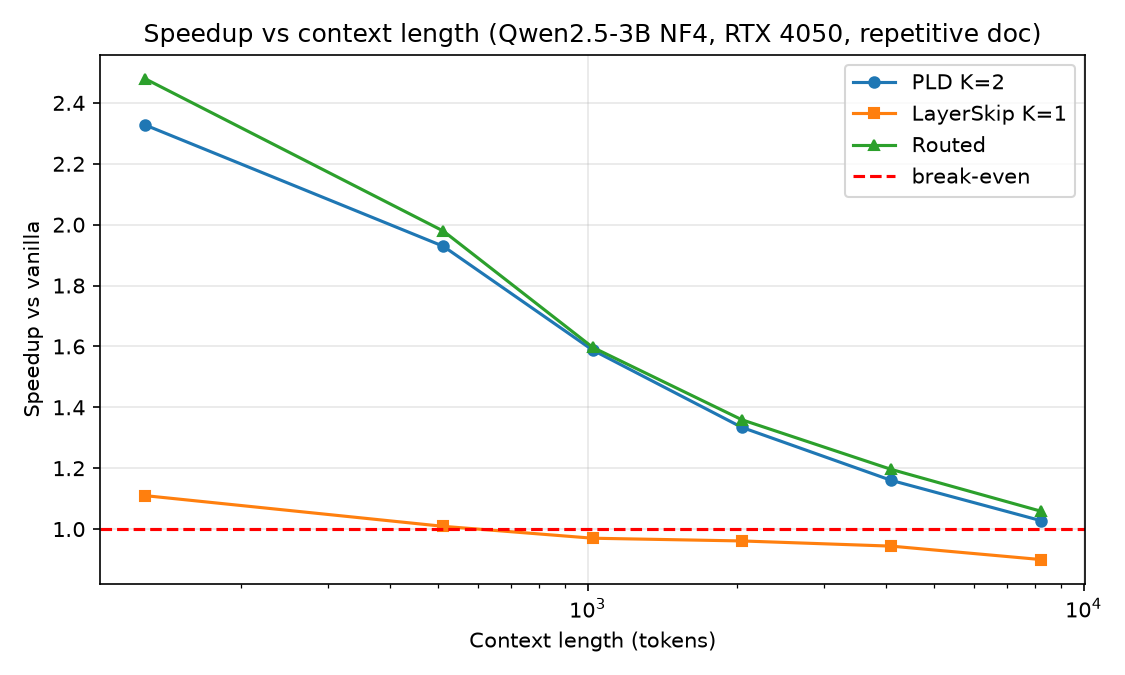
\includegraphics[width=\columnwidth]{../figures/context_sweep.png}
\caption{Speedup vs.\ context length (repetitive doc, Qwen2.5-3B NF4, RTX~4050). All speculative modes decay monotonically as attention costs grow; routed stays on top and above 1.0$\times$ through 8K while layer-skip falls below unity past 1K---consistent with a feasibility boundary that shifts with context length. Note: this repetitive-doc slice reaches $\sim$1.1$\times$ for layer-skip $K{=}1$ at $\sim$128 tokens via very high $\alpha$, unlike GSM8K sweeps (Sec.~\ref{sec:sweep_corr})---workload dependence, not contradiction.}
\label{fig:ctxsweep}
\end{figure}

\subsection{Router Ablation}
\label{sec:ablation}

Rule-level ablation on GSM8K-$N{=}50$ (fresh router per config) ranks the rules by necessity: removing the feasibility gate drops 1.070$\times{\to}$0.987$\times$ (gate contribution $+0.083$, the \textbf{core mechanism}); removing the PLD margin costs only $-0.008$ (\textbf{minor tie-break}); removing weak-hit capping ($+0.026$) or horizon tuning ($+0.095$) \textit{helps} on this highly-repetitive math workload, where long PLD verifies pay off---R1/R4 are \textbf{workload-dependent robustness heuristics} (safety on generic text), not universal improvements. (\texttt{experiments/16\_hybrid\_roofline/router\_ablation.json}.)

Starting from naive fallback (overall 1.002$\times$): asymmetric PLD margin (R2) + weak-hit capping (R1) reach 0.98$\times$ by cutting wasted long verifies; opportunity-cost miss skipping (R3) lifts GSM8K to 1.12$\times$ by replacing 0.88$\times$ LS cycles with 1.0$\times$ vanilla steps; adaptive PLD horizon (R4) stabilizes the mean at 1.020$\times$ ($N{=}10$ tuning runs; 1.063$\times$ at $N{=}50$). Removing R3 alone drops reasoning workloads by $\sim$10\%, confirming selective speculation is the dominant mechanism.

\section{Limitations}
\label{sec:limitations}

(i)~GSM8K is extended to $N{=}200$, HumanEval to full-164, CNN/DM to $N{=}200$ (combined: routed 1.026--1.081$\times$, all $p{<}0.001$ vs vanilla); short 48-token greedy generations favor PLD; new free-form (6 prompts, 96 tokens) and 256-token runs still favor PLD (1.05--1.44$\times$), so multi-seed and a true PLD-losing workload remain future work; (ii)~only the RTX~4050 rows are measured, cross-GPU rows in the appendix are idealized $1/\mathrm{BW}$ projections with assumed $\rho$ contradicted by Nsight on NF4 (calibration script: \texttt{scripts/run\_cross\_gpu\_calibration.py}); achieved streaming is $\sim$36--85~GB/s depending on byte accounting with kernel breakdown in Sec.~\ref{sec:aux}; no second backend (CUDA graphs/torch.compile/Marlin/AWQ/vLLM/llama.cpp) tested; (iii)~greedy decoding only---sampling-mode distribution tests are future work; (iv)~on this stack layer-skip always loses, so the optimal policy here is PLD plus vanilla fallback, i.e.\ pure PLD (1.144$\times$ vs routed 1.063$\times$); the gate's $+0.083$ is measured against layer-skip fallback and is conceptually close to SmartSpec goodput gating~\cite{smart2024spec}; the router's edge is only versus fixed layer-skip, not versus PLD; (v)~7B feasibility is shown via measured weight accounting plus a 1.5B-NF4 near-boundary case (62.9~MB headroom), not end-to-end 7B generation; auxiliary-draft throughput is now measured for 3B+0.5B NF4 ($N{=}18$, 1.058$\pm$0.031 at $K{=}2$, file \texttt{baseline05\_N18.json}) but not for 7B; (vi)~adapted KnapSpec/SpecBound are validated for ranking against the official KnapSpec code on shared hardware (Sec.~\ref{sec:official}), but SpecBound has no official runnable artifact in our stack and official-KnapSpec validation is only Llama-1B FP16, AIME24, $N{=}8$; exact-match gap (60\% sequences vs $\sim$0.2\%/token audit) implies $\sim$1.6\%/token on true trajectories---8$\times$ the isolated audit---and needs teacher-forced FP16 comparison.

\section{Reproducibility}
\label{sec:repro}

All claims are reproducible from the release: \texttt{reproduce.sh --quick} re-runs unit tests (81/81), roofline calibration, router simulation, margin/robustness sweeps, and benchmark statistics on CPU in $\sim$2~min; the full GPU path re-runs the $N{=}50$ suite ($\sim$1~h on an RTX~4050). A pinned \texttt{Dockerfile} (PyTorch~2.11/CUDA~12.8), per-experiment JSON with raw per-sample rows, ID-aligned paired-test scripts, and model-exact \texttt{requirements}/\texttt{pyproject} are included. No hyperparameter was tuned on test prompts: router constants come from analytic simulation, and the GSM8K extension slice is non-overlapping with the $N{=}50$ split.

\section{Conclusion}
\label{sec:conclusion}

Zero-weight speculation is \textit{feasible} on 6~GB GPUs, layer-skip self-speculation at $c{\approx}0.77$--0.82 is \textit{not faster} there by the geometric bound $(1{+}\alpha)/(1{+}c)$ (NF4 kernel inefficiency compounds but does not create the bound), and a cost-aware router over retrieval drafting plus selective vanilla skipping recovers consistent $>1.0\times$ speedups on Qwen, though still below pure PLD (1.063$\times$ vs 1.144$\times$); on this stack the optimal policy is PLD plus vanilla fallback. Two anchors carry the thesis beyond our own code: the \textit{official} FP16 KnapSpec reproduces 0.86$\times$ at 97.8\% acceptance near the bandwidth bound---acceptance is not speedup, by high $c$ rather than kernel inefficiency there---and the 128--8K context sweep shows monotonic decay with context consistent with rising attention cost, with a $\sim$1.1$\times$ layer-skip point at $\sim$128 tokens on highly repetitive text via very high $\alpha$. The cost model (in-device MAPE 2.4\%) quantifies when each technique wins on this measured stack; cross-GPU $1/\mathrm{BW}$ rows are an idealized bound contradicted by Nsight and retained in the appendix for illustration only.

\bibliographystyle{plain}
\bibliography{references}

\end{document}
